\documentclass[12pt]{article}

%Allgemeine Einstellungen

%Abstände
\usepackage[a4paper,left=3cm,right=3cm,top=3cm,bottom=3.5cm,headsep=12pt]{geometry}%Bottom extra 0.5cm für Footer

%Deutsches Sprachpacket
\usepackage[german,ngerman]{babel}

%Times New Roman
\usepackage{mathptmx}

%Titelseite einbinden
\usepackage{pdfpages}

%1.5-Zeilenabstand
\usepackage[onehalfspacing]{setspace}

%Stil der Überschriften, siehe ueberschriften.sty
\usepackage[numeric]{ueberschriften}

%Stil des Inhaltsverzeichnisses, siehe inhaltsverzeichnis.sty
\usepackage[numeric]{inhaltsverzeichnis}

%Abkürzungsverzeichnis, siehe abk_verzeichnis.sty
\usepackage{abk_verzeichnis}

%Stil der Fußzeilen, siehe fusszeilen.sty
\usepackage{fusszeilen}

%Literaturverzeichnis und Zitate, siehe literatur.sty
\usepackage{literatur}

%Stil für Header und Footer, siehe header_footer.sty
%Wenn nicht erwünscht, müssen auch die Befehle \frontmatter, \mainmatter auskommentiert werden
\usepackage{header_footer}

%Stile für Code-Ausschnitte, siehe codes.sty
\usepackage{codes}

%Stile für Anhänge, Bilder, ...
\usepackage{anhang}

%Silbentrennung (manche Worte werden am Zeilenende nicht getrennt, diese müssen dann nachgetragen werden)
\usepackage[T1]{fontenc}
\hyphenation{öf-fent-lich-en}

%DEBUGGING (Zeigt Boxen an)
%\usepackage{showframe}

\begin{document}

\renewcommand{\mytitle}{Governanceethik und\\moralische Anreize}%Titel für oben links
\renewcommand{\myauthor}{Lennart Schulte-Kellinghaus,\\Timo Stovermann}%Name für unten links
\renewcommand{\headheight}{27pt}%Bei Mehrzeiligem Titel muss Headerhöhe angepasst werden


\includepdf[pages={1-}]{titelseite.pdf}

\frontmatter%Stil des Headers/Footers ändern

\pagenumbering{Roman}

\addcontentsline{toc}{part}{Abkürzungsverzeichnis}%Abk-Verz. ins Inhaltsverzeichnis
\printabbreviations%abk_verzeichnis.sty
\clearpage
\renewcommand{\plaintitle}{Inhaltsverzeichnis}%Titel für oben Rechts
%Defbox, damit gepunktete Linie bis zur Zahl geht
{\def\makebox[#1][#2]#3{#3}%
	\tableofcontents
}

\addtocontents{toc}{\vspace{24pt}}%Freiraum im ToC

\clearpage
\mainmatter%Stil des Headers/Footers ändern
\pagenumbering{arabic}

\part{Theoretische Grundlagen}
Ethik spielt in Unternehmen eine immer größer werdende Rolle. Im Kontrast zum 20. Jahrhundert, als beispielsweise hohe Emissionswerte eines Unternehmens kaum Beachtung gefunden haben, gehen die CO2-Emissionen von Unternehmen seit Jahren stetig zurück. Genauso hat die Gleichberechtigung von Männern und Frauen immer mehr Präsenz in der Wirtschaft gewonnen, in form von Anstrengungen den Gender-Pay-Gap zu eliminieren oder den Frauenanteil in Management-Positionen zu erhöhen. Diese beiden Veränderungen sind neben vielen anderen maßgeblich durch Ethik bestimmt, da sie keinen (direkten) wirtschaftlichen Nutzen schaffen. In wie fern die Ethik und gesellschaftliche wie moralische Aspekte die Entscheidungen eines Unternehmens beeinflusst, soll hier kurz erörtert werden.
\section{Governance}
Gegenüber der klassischen Unternehmensführung versteht man unter dem Begriff Governance nicht-hierarchische Formen der Steuerung, in denen eine Verknüpfung verschiedener Ebenen und Perspektiven im Fokus steht. Im wirtschaftlichen Kontext wird der Begriff Corporate Governance auf Prinzipien innerhalb eines Unternehmens angewendet, welche den rechtlichen und faktischen Ordnungsrahmen für die Leitung und Überwachung festlegen. Der Zweck dieser Prinzipien ist es, Interessenkonflikte zwischen Shareholdern und Stakeholdern zu schlichten und das Unternehmen für alle Akteure ansprechend zu gestalten, um opportunistisches Verhalten einzuschränken. Dabei spielen neben ökonomischen auch moralische Anreize eine Rolle.
\section{Systemtheoretische Zusammenhänge}
Die wirtschaftliche wie soziale Gesellschaft besteht aus vielen Teilbereichen, welche teilweise unterschiedliche Ansichten zu den gleichen sozio-ökonomischen Fragestellungen vertreten. Ein solches Funktionssystem hat jeweils einen “Leitcode”, eine Sprache, über welche es gesteuert wird. Bei der Wirtschaft ist dies der Angebot-Nachfrage-Mechanismus mit dem Kommunikationsmittel Geld. Ein Funktionssystem kann nur über seinen Leitcode kommunizieren, was das Zusammenwirken von mehreren Funktionssystemen zur selben Problematik zunächst unmöglich macht. Daraus folgt, dass die Moral als Zweck an sich im reinen Wirtschaftssystem keinen Platz hat, da sie an sich keine monetäre Wertschöpfung bewirkt. Deshalb wird neben den Funktionssystemen das Konstrukt der Organisationssysteme eingeführt. Diese sind in der Lage, mit mehreren Funktionssystemen zu kommunizieren und Diskurse zwischen diesen zu moderieren.
\section{Die Anreiz-Dimensionen}
Anreize können anhand zweier Dimensionen kategorisiert werden, der Art der primären Hintergründe und die Herkunft des Anreizes. Die Hintergründe können ökonomisch, also primär auf das Eigeninteresse des Unternehmens bezogen, sein oder moralisch, welche “nicht nur aufgrund externer Belohnung [...] befolgt” werden sondern auf gesellschaftlichen Normen basieren. Auf der zweiten Dimension können externe Akteure (Kunden, Partner, Staat, …) oder unternehmensinterne Beweggründe einen Anreiz hervorrufen bzw. belohnen. Daraus ergibt sich eine Matrix mit 4 Anreiz-Kategorien.
\begin{center}
\begin{tabular}{|p{3cm}|p{5cm}|p{5cm}|}
\hline
Anreize & \textbf{extrinsisch} & \textbf{intrinsisch}\\\hline
\textbf{ökonomisch} & extrinsisch-ökonomisch & intrinsisch-ökonomisch\\\hline
\textbf{moralisch} & extrinsisch-moralisch & intrinsisch-moralisch\\\hline
\end{tabular}
\end{center}
\part{Treiber moralischen Handelns}
Der jeweilige Stellenwert bzw. überhaupt die Existenz der in 1.3 aufgezeigten Kategorien im System der Governance ist unter Ökonomen und Philosophen strittig. Grob lassen sich zwei Sichtweisen erkennen, die monistische und die dualistische.
\section{Die monistische Sichtweise}
Nach der monistischen Ansicht sind die Problemstellungen von Ethik und Ökonomik im Grunde deckungsgleich. Der Soziologe Amitati Etzioni argumentiert, dass moralisches Verhalten nicht auf ein Anreizsystem zurückführbar sei. Vielmehr sei es gleichermaßen durch ökonomische und moralische Erwartungen bestimmt, die letztenendes alle auf ökonomische Ziele abgestellt sind. Nach dieser Ansicht wäre der Rückgang von industriellen CO2-Emissionen darauf zurückzuführen, dass die Unternehmen so ihren Kundenkreis sichern und erweitern wollen, da erwartet wird, dass die Kunden die ethische Dimension des Umweltschutzes bei ihrer Kaufentscheidung mit einbeziehen.\\
\\
Der Ökonom Karl Homann beschreibt den weitergehenden Standpunkt, dass die Betriebswirtschaftslehre in sich bereits moralisch richtig sei. Demnach lägen für fast alle ethischen Probleme ökonomische Rekonstruktionen vor und die Ökonomik sei sogar in der Lage, ethische Probleme zu lösen, da diese in letzter Instanz auch nur auf individuellen Kalkülen basieren. Die Gründe dafür sieht Homann zum einen in der unter 1.2 beschriebenen funktionalen Differenzierung der Gesellschaft, zum anderen in der Beschaffenheit des Menschen als vollständig rational und nutzenorientiert handelnden “homo oeconomicus”.\\
\\
Wenn wir versuchen, die Anreize-Matrix aus 1.3 im monistischen Sinne zu füllen, kommennur extrinsich-ökonomische und intrinsisch-moralische infrage, da sämtliche ökonomisch relevanten Anreize auf eine materielle Vorteilskalkulation zurückführbar sind und der materielle Gewinn durch die externe Partei der Kunden bestimmt wird während alle immateriellen Anreize sich auf die Präferenzen der Akteure im Unternehmen beziehen und ohne monetären Vorteilseffekt sind.
\begin{center}
\begin{tabular}{|p{3cm}|p{5cm}|p{5cm}|}
\hline
Anreize & \textbf{extrinsisch} & \textbf{intrinsisch}\\\hline
\textbf{ökonomisch} & materiell\newline(Gewinnmaximierung, Markenimage, ...) & /\\\hline
\textbf{moralisch} & / & immateriell\newline(Sinn für Gerechtigkeit, Überzeugungen, ...)\\\hline
\end{tabular}
\end{center}
Der Versuch, immaterielle Anreize in die ökonomische Kalkulation mit einzubeziehen, würde demnach nur “Rauschen in der Wirtschaft” hervorrufen, indem sie für das Wirtschaftssystem irrelevante Diskussionen provozieren.
\section{Die dualistische Sichtweise}
Aus dem Wesen der monistischer Sichtweise folgt, dass sämtliche Handlungen eines (wirtschaftlichen) Akteurs durch andere Akteure bestimmt sind, unabhängig davon, ob sie materieller oder immaterieller Natur sind. Der dualistische Ansatzform geht im Gegensatz dazu davon aus, dass moralische und ökonomische Beweggründe einzeln zu betrachten sind und vor allem nicht immer miteinander einhergehen. Primär wird an dieser Stelle die Governanceethik von Josef Wieland betrachtet, welche ein umfassendes Konzept zur Berücksichtigung genuiner moralischer Anreize in Governancestrukturen liefert.
\subsection{Das Anreizsystem nach Wieland}
Für Wieland beschränken sich moralische Anreize nicht bloß auf die intrinsischen Aspekte, da Achtung und Mißachtung von der Gesellschaft zwar nicht um ihrer selbst Willen verliehen werden aber dennoch moralischer Natur seien. Des weiteren können immaterielle Anreize ebenso von intern heraus entstehen, wie zum Beispiel die Unternehmenskultur.
\begin{center}
\begin{tabular}{|p{3cm}|p{5cm}|p{5cm}|}
\hline
Anreize & \textbf{extrinsisch} & \textbf{intrinsisch}\\\hline
\textbf{ökonomisch} & materiell\newline(Gewinnmaximierung, ...) & immateriell\newline (Eigeninteresse, Identifikation, ...)\\\hline
\textbf{moralisch} & immateriell\newline (Achtung, Anerkennung) & immateriell\newline(Sinn für Gerechtigkeit, Überzeugungen, ...)\\\hline
\end{tabular}
\end{center}
Die vier Anreizformen treten auf unterschiedliche Art in Erscheinung. Extrinsich-ökonomische Anreize sind von außen determinierte materielle Kalkulationen wogegen extrinsich-moralische Anreize nicht auf monetären Zielen sondern auf dem immateriellen Bedürfnis des Menschen nach Anerkennung und Achtung durch Mitmnschen basieren. Die intrinsich-moralischen Anreize stellen die Anreize dar, die befolgt werden um ein inneres Bedürfnis zu erfüllen, (Vgl. 1.4) und intrinsich-ökonomische Anreize sind interne Anforderungen an das Unternehmen als Wirtschaftlichen Akteur, wie zum Beispiel eine Unternehmenskultur.
\subsection{Die Bedeutung von Moral in der Wirtschaft}
In der Governanceethik wird neben den ökonomischen Gütern die Kategorie der moralischen Güter eingeführt, bei denen nicht Preis-Leistung sondern die moralische Legitimität den Ausschlag gibt. Da sich diese in ihrer Grundlage von anderen Wirtscahftsgütern unterscheiden und im Zweifelsfall auch ein Stück Kleidung zu einem Moralgut werden kann, z.B. wenn öffentlich wird, dass es unter Kinderarbeit hergestellt wurde, ist es essentiell, dass ein Unternehmen den Umgang mit moralgütern definiert.\\
\\
Die Kernessenz der Moralgüter liege in der sozialen Kooperation von Menschen und Unternehmen. Kein Vertrag und keine Vereinbarung deckt sämtliche Szenarien zu 100\% ab. Und in eben dieser Unsicherheit kommen extrinsisch-moralische Anreize zum tragen, da diese dem Akteur Achtung und Misachtung für vertraglich nicht geregelte Handlugnen zurechnen und so ein Vertrauensverhaltnis zwischen Akteuren schaffen. Die intrinsich-moralischen Güter haben einen Einfluss, da eigene Überzeuungne, Werte und Haltungen sowie Selbstwertschätzung die Grundlage einer Identitätsbildung sind, welche wiederum die Grundlage zur sozialen Kooperation und Kommunikation sei, welche die Grundvoraussetzung zur Allokation von WErtschätzung ist. Dier Kernessenz der Moral im Wirtschaftssystem nach Wieland ist also, dass eine wirtschaftliche Transaktion nicht nur eine materielle Wertsteigerung bewirken soll, sondern auch eine Steigerung der externen und internen Wertschätzung.

\subsection{Governanceethik nach Wieland}
Genau in der Wertschätzung liegt die Kernessenz von Wielands Governanceethik, da diese als Kommunikationsmedium des damit vollständigen Funktionssystems “Moral” fungiert. Dieses Funktionssystem kann dann als genuiner Bestandteil der Organisationssystems Unternehmen agieren und somit können moralische Anreize, ob intrinsich oder extrinsich, ein integraler Bestandteil der Governance werden. Das Zusammenspiel beider Funktionssysteme wird in folgender Grafik visualisiert:
\begin{center}
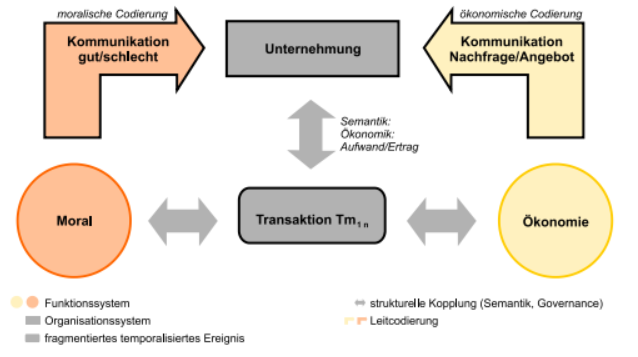
\includegraphics[width=.75\textwidth]{wieland1.png}
\end{center}
Jede wirtschaftliche Transaktion hat eine ökonomische und eine moralische Dimension, deren Gewichtung sowohl von der Identität des Unternehmens als auch von der gegebenen Situation abhängig ist. Wieland fasst den moralischen Transaktionsmechanismus in folgender Formel zusammen:
\[T_{mi}=f_{(aIS_i, bFI_{ij}, cIF_{ij}, dOKK_i)}\]
Das erste Argument der Formel ist die individuelle Selbstbindung  IS des Unternehmens, also die o.g. Identität. Ihr Einfluss bestimmt, ob das Ergebnis der Transaktion eher der Tugendethik oder einem rationalem Vorteilskalkül entspricht.\\
Der zweite Einflussfaktor sind die formalen Institutionen FI. Diese umfassen den gesetzgebenden Staat, Gewerkschaften oder ähnliches.\\
Die informalen Institutionen IF bilden das dritte Argument der Formel. Sie umfassen moralische und religiöse Überzeugungen einer gegebenen Kultur. An diesem Argument setzen also auch die extrinsisch-moralischen Anreize an.\\
Den letzten und für die Governanceethik bedeutensten Faktor stellen die Koordinations- und Kooperationsmechanismen des Organsiationssystems OKK dar. Darunter sind Leitlinien und Prozesse zu verstehen,mit denen moralische Anforderungen, wie Verzicht auf Kinderarbeit und Korruption operationalisiert und implementiert werden. Sie haben also einen Einfluss auf extriisch- und intrinsich-moralische Anreize.\\
Die PArameter a bis d können jeweils den Wert 1,0 odr -1 annehmen. Der Wert 1 gibt eine positive Wirksamkeit im Hinblick auf die moralische Dimension an. Der Wert -1 gibt genau das Gegenteil an, nämlich eine negative Wirkung auf die moralische Transaktion und der Wert 0 besagt, dass eine Wirkung nicht angenommen wird.
\section{Einordnung in philosophische Landschaft}
Die monistische Sichtweise lässt sich gut in den Utiliarismus einordnen,da hier der Gesamtnutzen der Gesellscahft unter der Annahme, dass ökonomisches Verhalten eben dies bewirkt, maximiert werden soll. Mit den Argumenten der Transaktion ergeben sich in der dualistischen Sichtweise folgende Kombinationsmöglichkeiten:
\begin{center}
\begin{tabular}{|p{4cm}|p{2cm}|p{2cm}|p{2cm}|p{2cm}|}
\hline
 { } & IS & FI & IF & OKK\\\hline
 Tugendethik & 1 & 0 ; -1 & 0 ; -1 & 0 ; -1\\\hline
 Ordnungsethik & 0 ; -1 & 1 & 0 ; -1 & 0 ; -1\\\hline
 Globale Ethik & 0 ; -1 & 0 ; -1 & 1 & 0 ; -1\\\hline
 Unternehmensethik & 0 ; -1 & 0 ; -1 & 0 ; -1 & 1\\\hline
\end{tabular}
\end{center}
Wenn sich das Handeln an den persönlichen Überzeugungen orientiert, ist das handeln tugendethisch. Ein schlichtes Gehorchen der formalen Institutionen entspricht der Ordnungsethik, welche moralisches Handeln durch Regelsetzung bewirken will. Wenn die globale Gesamtheit moralischer Normen mehr Beachtung als formale Regelungen oder die persönliche Entscheidung bekommt, liegt Globale Ethik vor. Und wenn die Governance-Systeme (OKK) die entscheidenend Instanzen darstellen, liegt reine Unternehmensethik vor.\\
\\
Die Tugendethik Immanuel Kants besagt im kategorischen Imperativ, dass eine moralische Handlung nicht nur “pflihtgemäß” sein muss, sondern auch “aus der Pflicht heraus” motiviert sein muss. Demnach wäre die Reduktion der CO2-Emmissionen mit dem Ziel der Imagesteigerung keine moralische Handlung, da die Begründung nicht “um ihrer selbst Willen” ist. Wieland sieht hier aber die Schwäche, dass moralische Handlungen, die aus der reinen Überzeugung, dass sie richtig sind, entstehen, eigentlich auch nur ein Bedürfnis des Menschen stillen sollen, nämlich das, in Einklang mit seinen natürlichen Regungen und dem gesellscahftlichen Habitus zu leben, und somit einen Selbstnutzen mit sich bringen. Zudem sei dieser Habitus nicht naturgegeben, sondern werde über einen sozialen LErnprozess vermittelt. Stattdessen entwickelte Wieland für die Unternehmensethik den organisatorischen Imperativ. Dieser besagt, dass ein Akteur so handeln soll, moralische Güter zu aktivieren und Opportunismus zu minimieren. Eben diesen Zweck sollen die moralsensitiven Governancestrukturen erüllen. In diesem Konstrukt werden Entscheidungen nicht mehr anhand des “homo oeconomicus” getroffen, sondern aus einer situativen Abwägung von Moral und Ökonomie.
\clearpage
\frontmatter%Stil des Headers/Footers ändern
\renewcommand{\plaintitle}{Literaturverzeichnis}
\pagenumbering{Roman}
\setcounter{page}{5}
\addtocontents{toc}{\vspace{24pt}}
\addcontentsline{toc}{part}{Literaturverzeichnis}%Literatur-Verz. ins Inhaltsverzeichnis
\printMyBibliography

\end{document}